\documentclass[12pt]{article}
\usepackage[a4paper, total={6in, 9in}]{geometry}
\usepackage{graphicx}
\graphicspath{ {./images/output/} }
\usepackage{caption}
\usepackage[english]{babel}
\usepackage{titling}
\usepackage{float}
\usepackage{amsmath}
\usepackage{minted}
% \usepackage{multicol}
% \usepackage{array}
% \usepackage{setspace}
% \usepackage{placeins}
\usepackage{parskip}

% \usepackage{lipsum}

\title{Implementation of CMOS Inverter.}
\author{}
\date{}

\pagenumbering{gobble}
\begin{document}
\vspace*{\fill}
\begin{center}

    \emph{Heaven's Light is Our Guide} \\
    \textbf{Rajshahi University of Engineering and Technology} \\

    \begin{figure}[H]
        \centering
        
\includegraphics[scale=.34]{images/RUET_logo.png}
        \label{fig:ruet_logo}
    \end{figure}
    \vspace{5mm}

    \textbf{Course Code}\\
    ECE 4128\\
    \vspace{3mm}
    \textbf{Course Title}\\
    VLSI Design

    \vspace{5mm}
    \textbf{Experiment Date:} {July 4, 2025},\\
    \textbf{Submission Date:} {August 11, 2025}\\

    \vspace{5mm}
    \textbf{Lab Report 2: \\
        Implementation of NMOS Ratio-less Inverter.}

    \vspace{15mm}

    \begin{tabular}{c|c}
        \textbf{Submitted to} & \textbf{Submitted by} \\
        Moloy Kumar Ghosh     &                       \\
        Lecturer              &                       \\
        Dept of ECE, RUET     & Md. Tajim An Noor     \\
        \&                    & Roll: 2010025         \\
        Md. Faysal Ahamed     &                       \\
        Lecturer              &                       \\
        Dept of ECE, RUET     &                       \\
    \end{tabular}

\end{center}
\vspace*{\fill}


\pagebreak

\tableofcontents

\pagebreak
\pagenumbering{arabic}
\maketitle

\section*{Theory}
\addcontentsline{toc}{section}{Theory}
A CMOS inverter is a fundamental building block in digital logic, consisting of a PMOS and an NMOS transistor connected in a complementary arrangement~\cite{rabaey2003digital}. The PMOS transistor is linked to the supply voltage (VDD), while the NMOS is connected to ground. Both transistors share the same input signal (Vin), and the output is taken from the junction between them. When the input is low (logic 0), the PMOS conducts and the NMOS is off, resulting in a high output (logic 1). Conversely, when the input is high (logic 1), the NMOS turns on, the PMOS switches off, and the output drops to logic 0. This complementary switching greatly reduces static power consumption, making CMOS technology highly energy efficient~\cite{kang2003cmos}.

An important dynamic property of CMOS inverters is the transition time, which includes rise time (tr) and fall time (tf). These times indicate how quickly the output voltage responds to changes in the input. Rise time refers to the interval during which the output increases from about 10\% to 90\% of VDD, while fall time measures the decrease from 90\% to 10\% of VDD. The speed of these transitions is crucial for high-speed digital circuits~\cite{weste2015cmos}.

\begin{figure}[H]
    \centering
    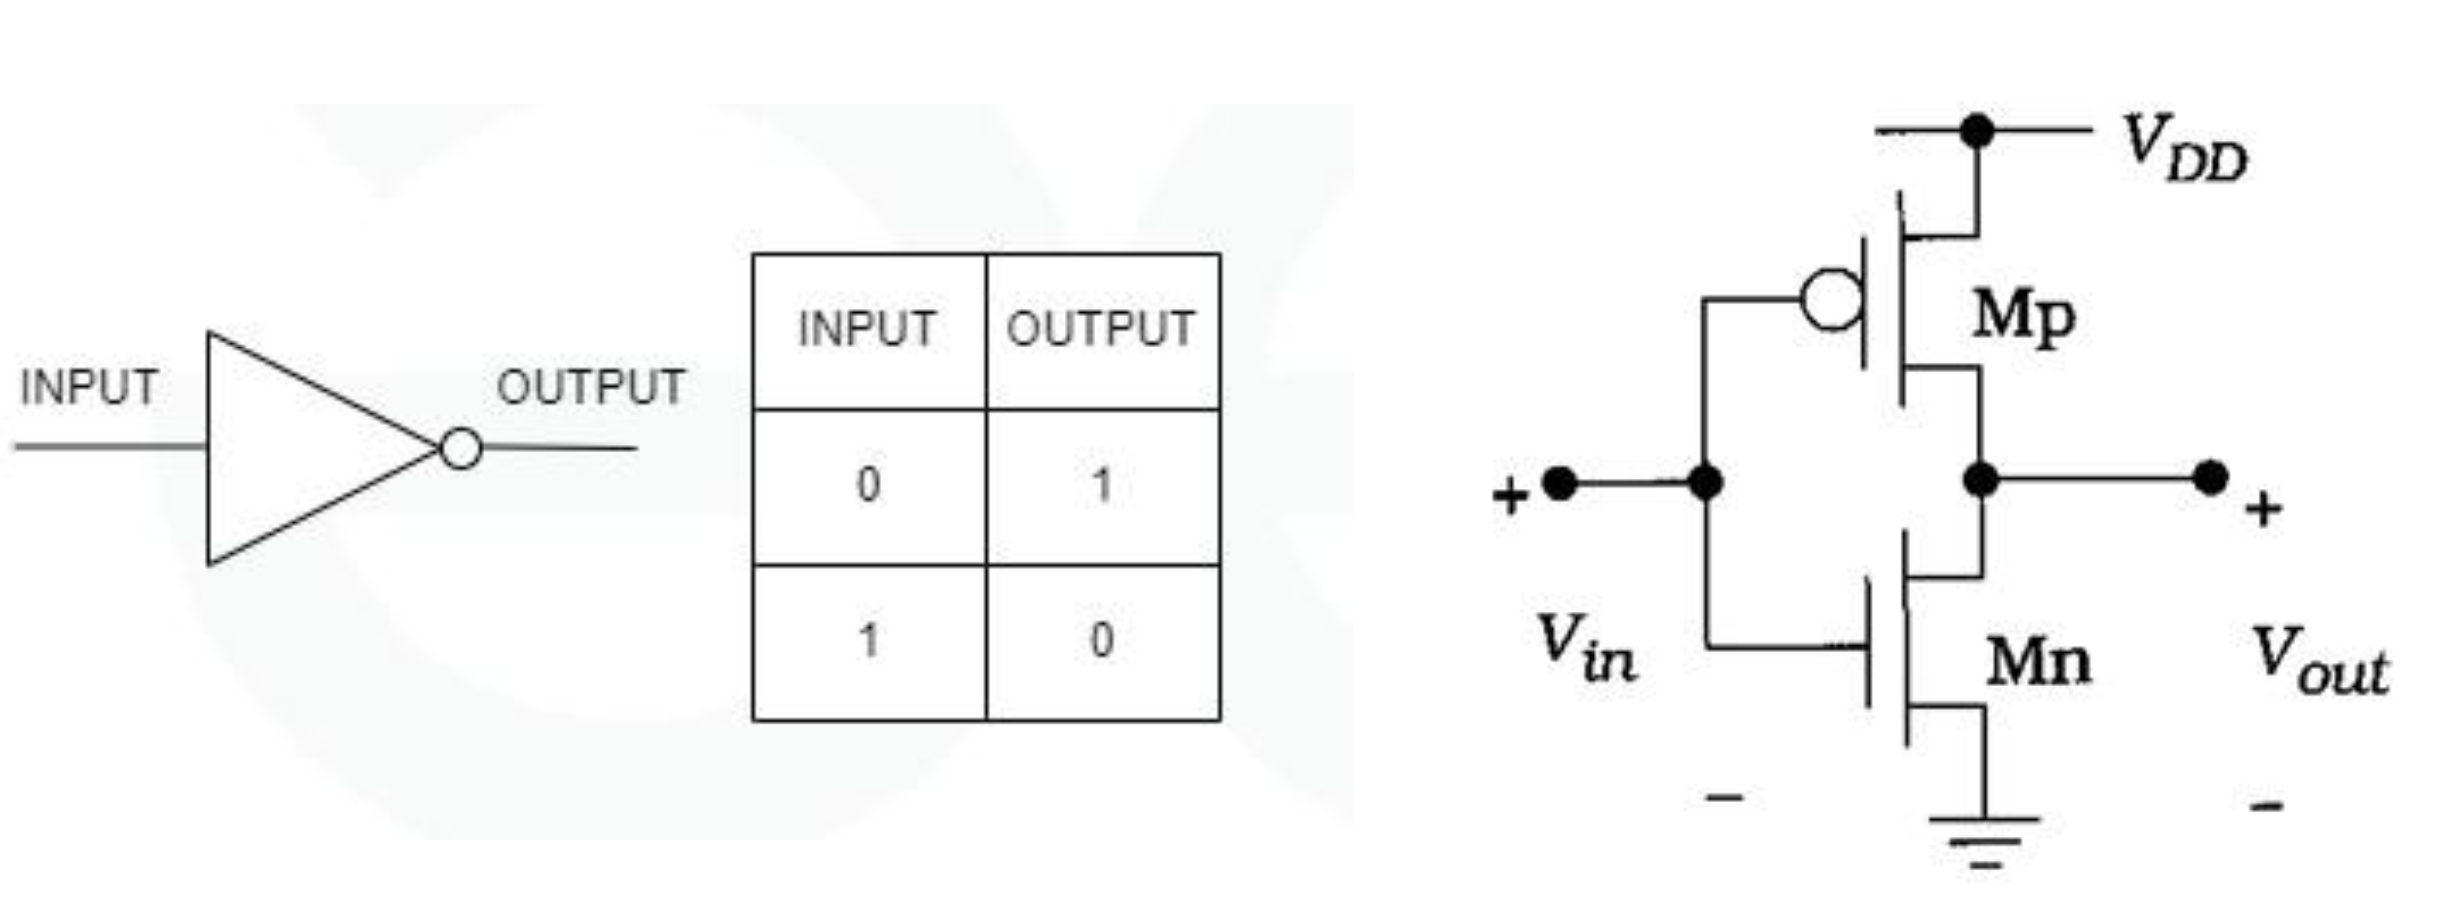
\includegraphics[width=0.8\textwidth]{th.png}
    \caption{Block diagram of a CMOS inverter circuit.\cite{GeeksforGeeks2025Jul}}
\end{figure}

The rise and fall times of a CMOS inverter depend on the output load capacitance ($C_{out}$) and the aspect ratios ($W/L$) of the transistors. Because PMOS transistors have lower carrier mobility ($\mu_p$) than NMOS transistors ($\mu_n$), the PMOS is usually made wider—often about twice the width of the NMOS—to equalize the speeds of the rising and falling edges~\cite{rabaey2003digital}. This matching is achieved when:
\[
    \frac{W_1}{L_1} \mu_n = \frac{W_2}{L_2} \mu_p
\]
where $T_1$ is the NMOS and $T_2$ is the PMOS. This relationship helps ensure that the inverter switches symmetrically.

The propagation delay due to the output capacitance can be approximated by:
\[
    t_r \approx 35 \cdot \frac{C_{out}}{W_1/L_1} \ \text{ns}
\]
where $C_{out}$ is in picofarads and $W_1/L_1$ is the NMOS aspect ratio. This means that larger output capacitance or smaller transistor sizes result in slower signal transitions~\cite{kang2003cmos}.

\section*{Required Tools}
\addcontentsline{toc}{section}{Required Tools}
\begin{itemize}
    \item Microwind
    \item MS Word
    \item \LaTeX
\end{itemize}

\section*{Circuit Schematic}
\addcontentsline{toc}{section}{Circuit Schematic}

\begin{figure}[H]
    \centering
    \begin{minipage}{0.48\textwidth}
        \centering
        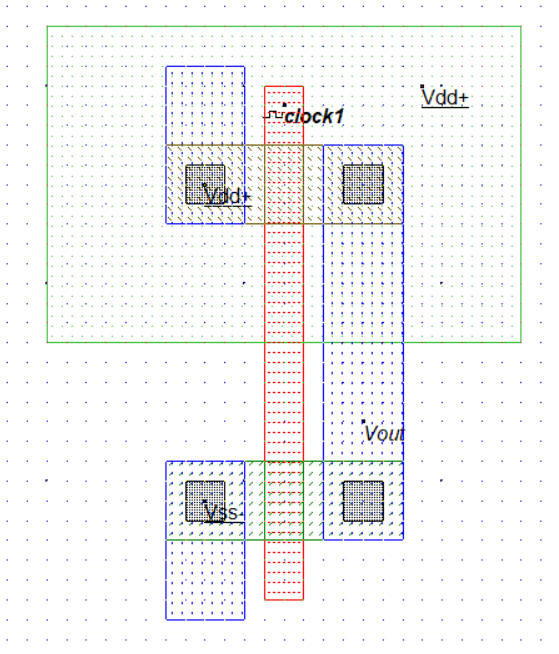
\includegraphics[width=\textwidth]{1inv.png}
        \caption{CMOS Inverter Schematic without Load Capacitor}
    \end{minipage}\hfill
    \begin{minipage}{0.48\textwidth}
        \centering
        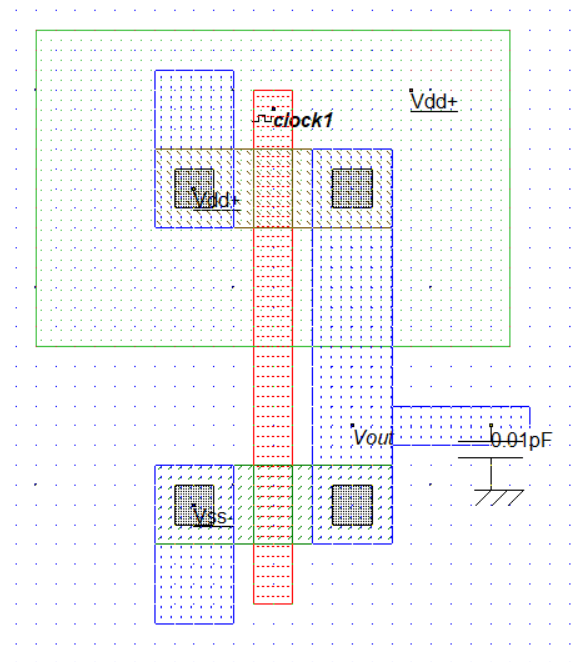
\includegraphics[width=\textwidth]{1cap_inv.png}
        \caption{CMOS Inverter Schematic with Load Capacitor}
    \end{minipage}
\end{figure}

\section*{Output}
\addcontentsline{toc}{section}{Output}

\begin{figure}[H]
    \centering
    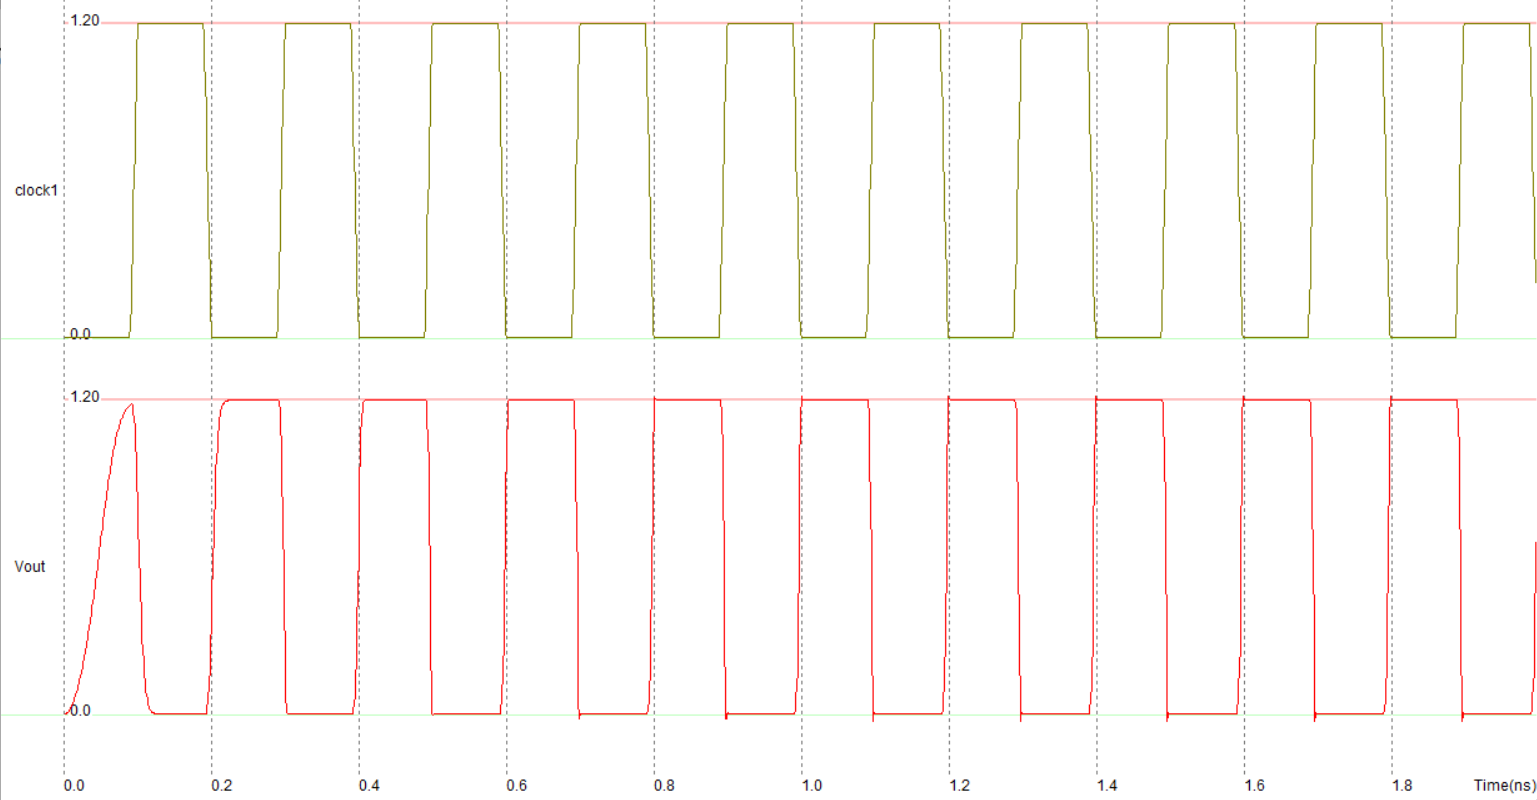
\includegraphics[width=0.75\textwidth]{11v_t.png}
    \caption{Plot of voltage over time without a capacitor.}
\end{figure}

\begin{figure}[H]
    \centering
    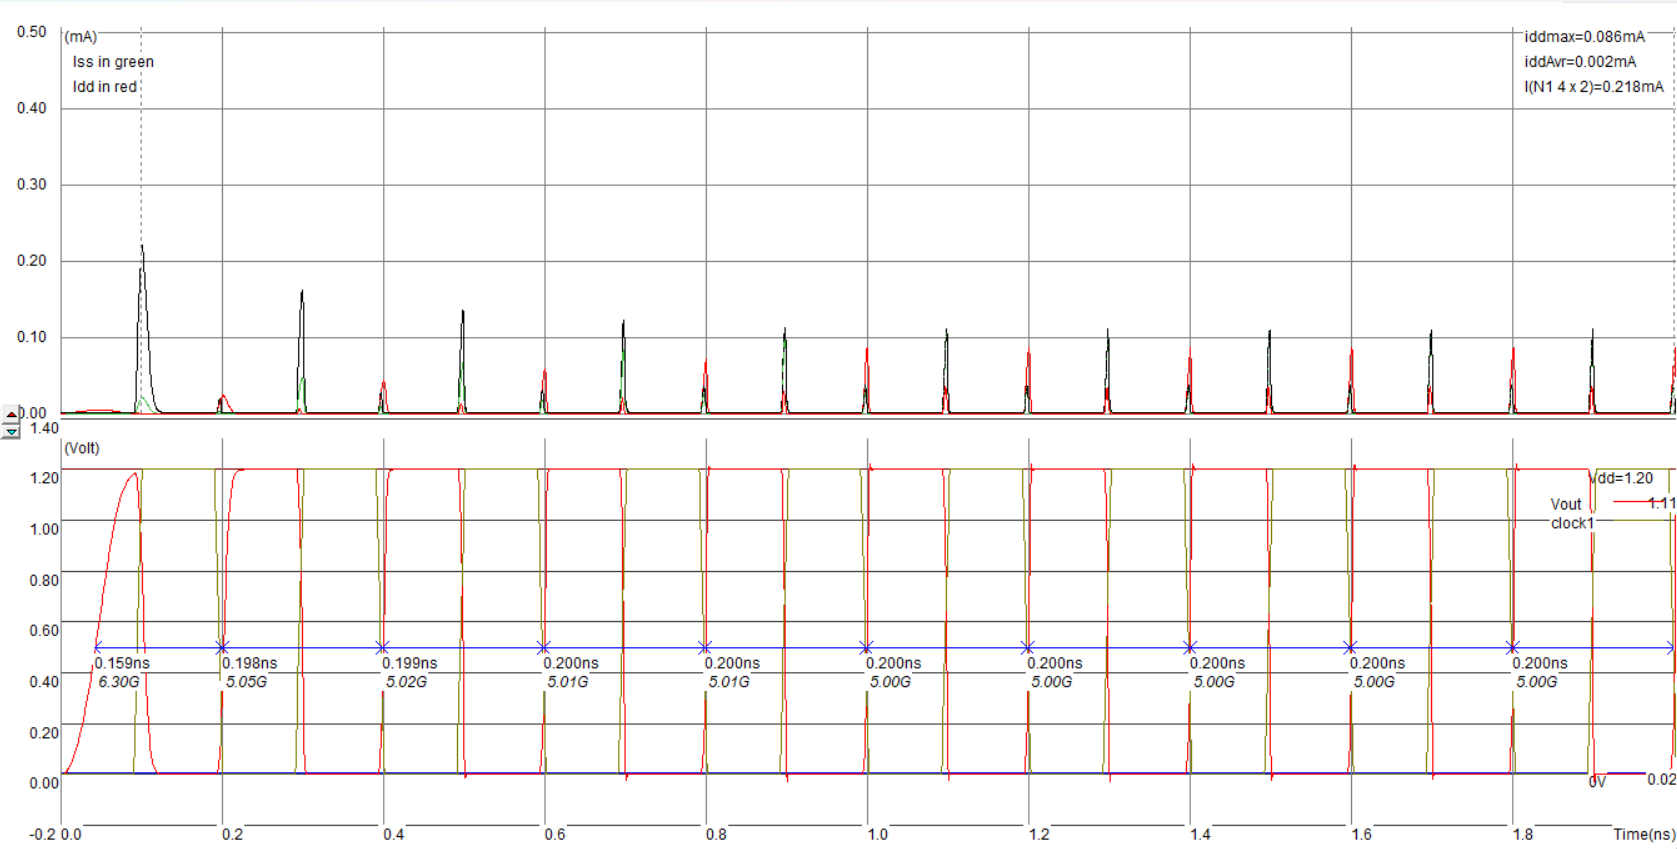
\includegraphics[width=0.75\textwidth]{21V_c.png}
    \caption{Plot of voltage versus current without a capacitor.}
\end{figure}

\begin{figure}[H]
    \centering
    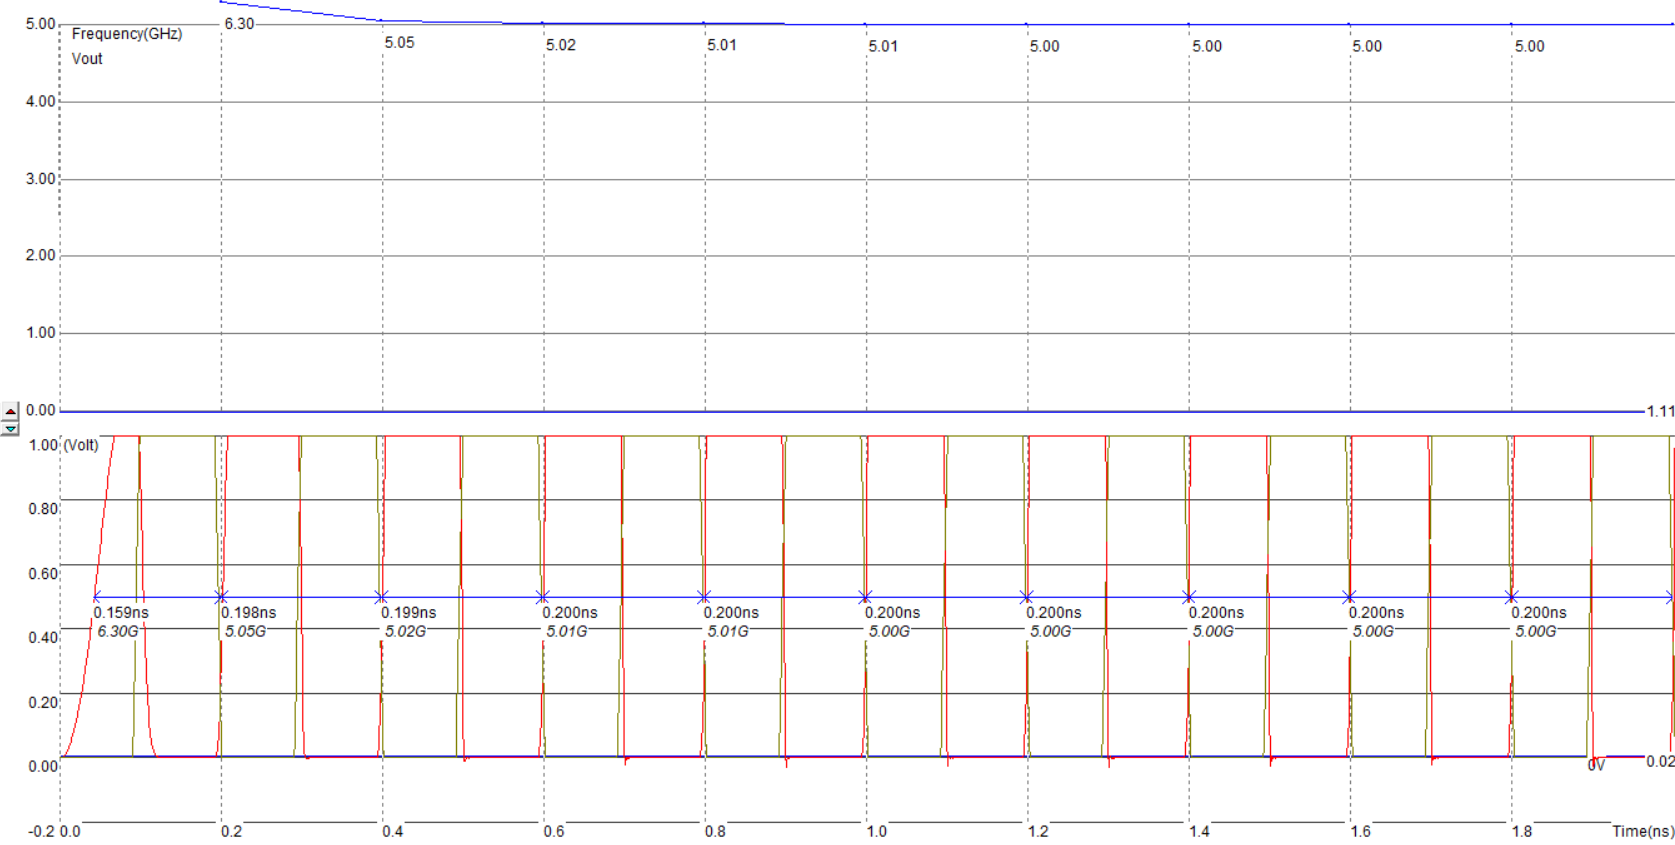
\includegraphics[width=0.75\textwidth]{31.png}
    \caption{Plot of frequency over time without a capacitor.}
\end{figure}

\begin{figure}[H]
    \centering
    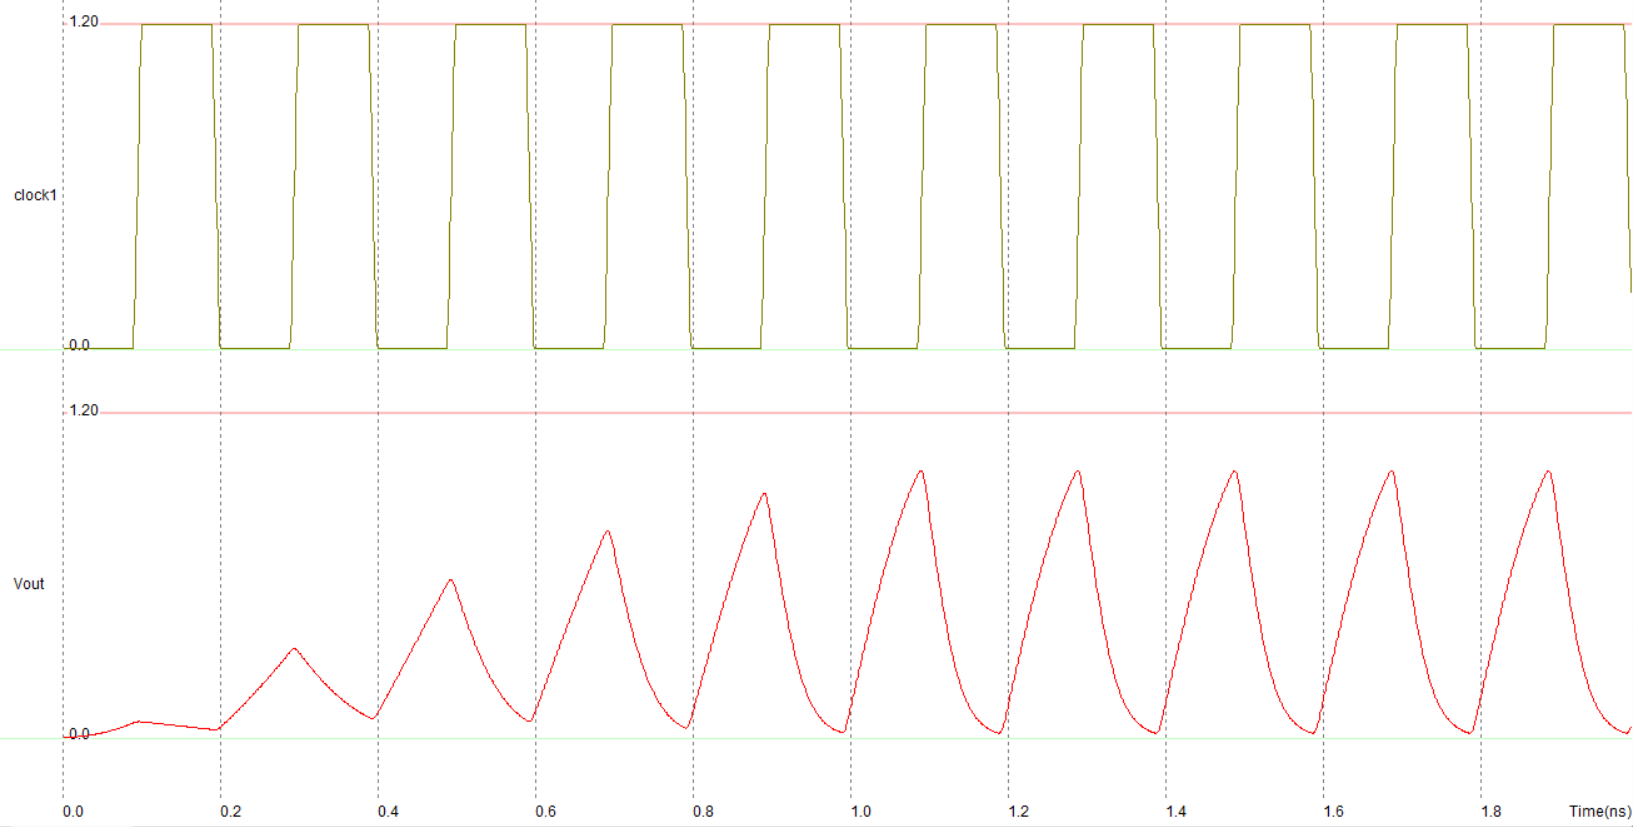
\includegraphics[width=0.75\textwidth]{41voltage_time.png}
    \caption{Plot of voltage over time with a capacitor.}
\end{figure}

\begin{figure}[H]
    \centering
    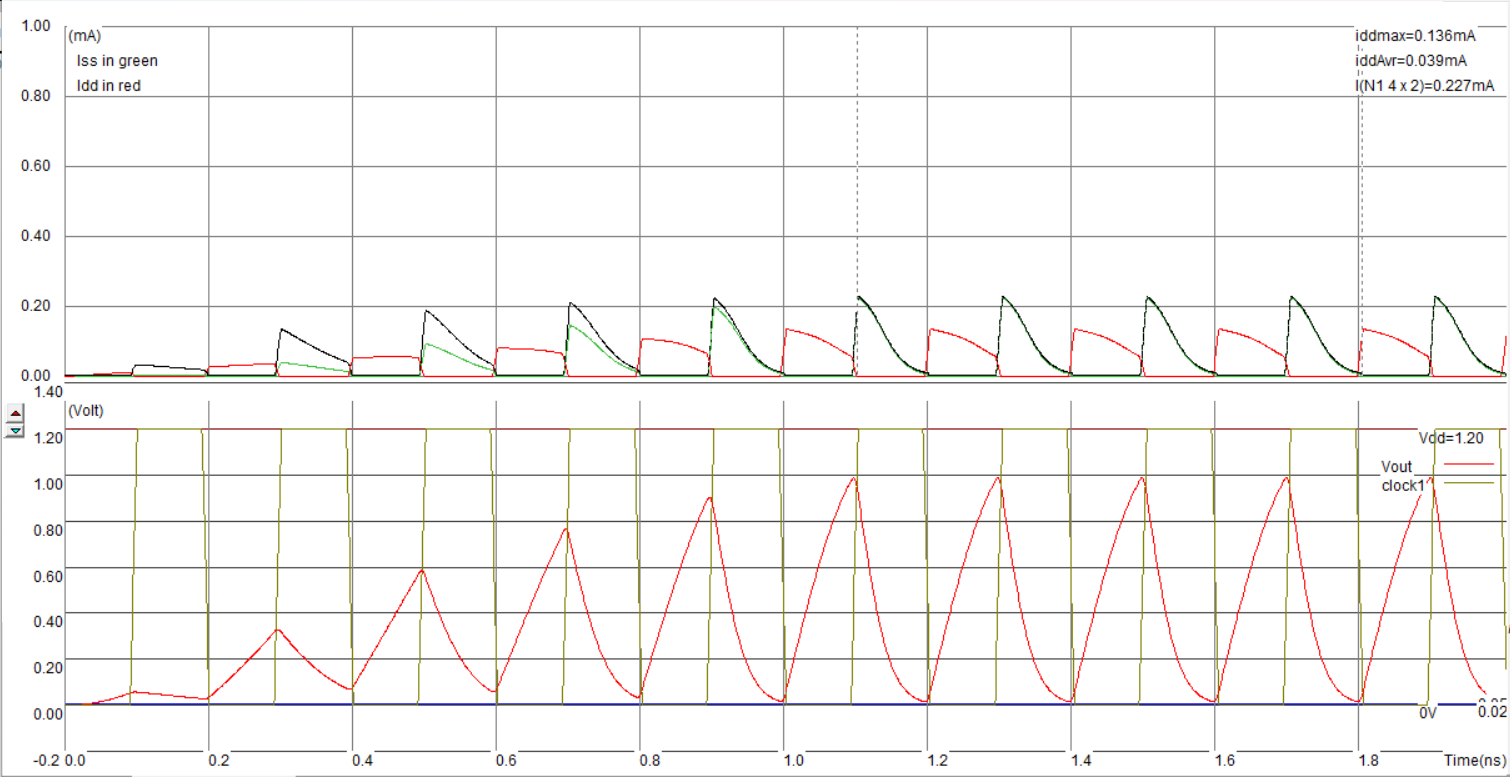
\includegraphics[width=0.75\textwidth]{51voltage_current.png}
    \caption{Plot of voltage versus current with a capacitor.}
\end{figure}

\begin{figure}[H]
    \centering
    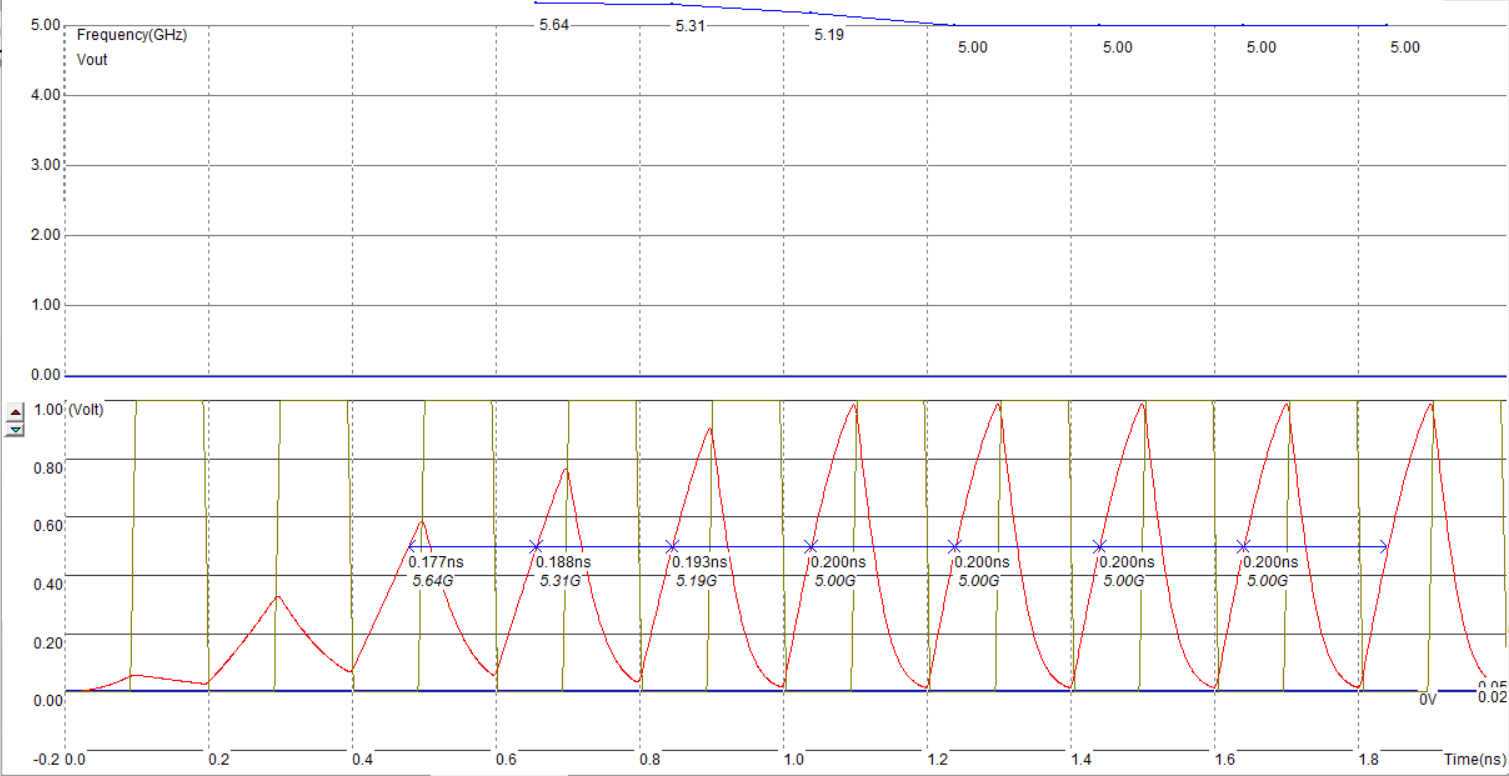
\includegraphics[width=0.75\textwidth]{61freq_time.png}
    \caption{Plot of frequency over time with a capacitor.}
\end{figure}

\section*{Discussion and Conclusion}
\addcontentsline{toc}{section}{Discussion and Conclusion}
This experiment involved designing and simulating a CMOS inverter in Microwind to analyze its switching behavior with a clocked input cycling between 0 V and 1.2 V. The simulation results verified the inverter’s basic function: the output reliably inverted the input signal. Various waveforms—including voltage versus time, current versus voltage, and frequency versus time—were examined for both unloaded and loaded output conditions.

Adding a load capacitor highlighted the rise and fall times, which stem from the charging and discharging of the output node, consistent with the relation $t_r = 35 \cdot C_{out}$ ns. In the absence of the capacitor, transitions appeared sharp and nearly ideal; with the capacitor, minor delays and current peaks were observed. These effects reflect fundamental CMOS principles, notably the impact of load capacitance and the necessity of balancing transistor dimensions to offset PMOS and NMOS mobility differences. Adjusting the aspect ratios achieved more symmetrical signal edges, enhancing timing characteristics.

In summary, the study confirmed theoretical expectations and practical behavior of CMOS inverters. It demonstrated that dynamic factors—such as output capacitance, transistor sizing, and carrier mobility—significantly influence propagation delay, switching speed, and power consumption. The findings reinforced the importance of careful design choices for efficient and robust VLSI circuits.

\bibliographystyle{IEEEtran}
\renewcommand{\bibname}{References}
\addcontentsline{toc}{section}{References}
\bibliography{ref}

\end{document}
